\section{Recovery Concepts}
\subsection*{1}
% In a system implementing force and no-steal, is it necessary
% to implement a scheme for redo? What about a scheme for undo? Explain why.
A system that implements force and no-steal will not have to implement a scheme
for undo or redo. On an aborted transaction the changes will not have been written to
disk yet, and on a committed transaction the changes are guaranteed to have been
written to disk at commit-time, so a subsequent crash does not matter.

\subsection*{2}
% What is the difference between nonvolatile and stable storage? What types of
% failures are survived by each type of storage?
Non-volatile storage is a storage medium that will retain its contents, even if
power is turned off. It is sometimes also referred to as \textit{stable storage}.
However, stable storage is often referred to as non-volatile storage that is
also coupled with some backup mechanism, in the context of recovery.

We assume here that stable storage is non-volatile storage, backed up both
locally and then copied to an external site. In such a case, we explore a few
different causes of failure and how they may affect the two different types of
storage, in Table~\ref{tbl:storage_types}.

\begin{table}[h!]
    \begin{tabular}{|l|c|l|}
        \hline
        \textbf{Failure type} & \textbf{Will non-volatile survive} &
        \textbf{Will Stable storage survive}
        \\ \hline
        Power outage & Probably & Yes (Data is backed up) \\ \hline
        Flood & Probably not & Yes (Data is backed up externally) \\ \hline
        Fire & Probably not & Yes (Data is backed up externally) \\ \hline
        Component failure & No & Yes (Data is backed up) \\ \hline
    \end{tabular}
    \caption{Failure types and survival assessment for non-volatile and stable
        storage.\label{tbl:storage_types}}
\end{table}

In general, disk loss is prevented from causing permanent data loss by
replicating disks and storing them elsewhere.

\subsection*{3}
A system implementing Write-Ahead Logging must force the log tail to stable
storage on two events:
\begin{enumerate}
    \item When a transaction is committed.
    \item When an update is undone, a compensation log record is written.
\end{enumerate}

\section{ARIES}
% 1) Transaction and dirty page table set to last checkpoint state. In this case
% blank.

% 2) Remove all transactions that have an end from the transaction table, as
% they are no longer active.

% 3) Add entries for the transactions that have not yet ended.
%  - Set lastLSN field to last LSN related to that transaction
%  - If the last record is a commit record, status is set to C, otherwise U to
%  signal it should be undone.

% 4) 

\subsection*{1}
The contents of the transaction table and dirty page table after the analysis
phase are:
\begin{table}[h!]
    \begin{tabular}{|l|l|l|}
        \hline
        transID & status & lastLSN \\ \hline
        T1 & U & 4 \\ \hline
        T2 & U & 9 \\ \hline
    \end{tabular}
    \caption{Transaction table.}
\end{table}

\begin{table}[h!]
    \begin{tabular}{|l|l|}
        \hline
        pageID & recLSN \\ \hline
        P2 & 3 \\ \hline
        P1 & 4 \\ \hline
        P5 & 5 \\ \hline
        P3 & 9 \\ \hline
    \end{tabular}
    \caption{Dirty page table}
\end{table}

\subsection*{2}
The winner transactions are those that completed, the loser transactions those
that are still in the transaction table. The \texttt{winners} = $\{T3\}$, the
\texttt{losers} = $\{T1,T2\}$.

% Sets of winner and loser transactions
\subsection*{3}
The redo phase begins at the $LSN$ of the record following the last checkpoint,
which in this case is $LSN=3$. The undo phase ends at $LSN=3$, as it scans
backwards.
% Values for the LSNs where the redo phase starts and where the undo phase ends
\subsection*{4}
Log records with the following LSN may cause pages to be rewritten during redo
phase: $\{3, 4, 8, 9\}$.
% Sets of log records that may cause pages to be rewritten during the redo phase
\subsection*{5}
Log records undone during the undo phase, in this order: $\{9,8,5,4,3\}$. ToUndo
will be initialized with the \texttt{lastLSN} of the loser transactions, namely
the LSNs $\{9, 4\}$. Then log records are undone in reverse order, starting from
the largest LSN (9).
% Set of log records undone during the undo phase
\subsection*{6}
% Contents of the log after the recovery procedure completes.
The contents of the log after the recovery procedure is complete, looks as
follows:

\begin{table}[h!]
    \begin{tabular}{|l|l|l|l|l|}
        \hline
        LSN & lastLSN & transID & type & pageID \\ \hline
        11 & 9 & T2 & CLR \{LSN=9, TID=T2, undoNext=8\} & N/A \\ \hline
        12 & 11 & T2 & CLR \{LSN=8, TID=T2, undoNext=5\} & N/A \\ \hline
        13 & 12 & T2 & CLR \{LSN=5, TID=T2, undoNext=4\} & N/A \\ \hline
        14 & 13 & T3 & CLR \{LSN=4, TID=T1, undoNext=3\} & N/A \\ \hline
        15 & 14 & T1 & CLR \{LSN=3, TID=T1, undoNext=None\} & N/A \\ \hline
    \end{tabular}
\end{table}

\section{Performance Measurements}
\textit{Note: Unfortunately, I was not able to get the remote benchmark to work
in time as I have been ill.}

\subsection*{1}
The data was generated using the \texttt{BookSetGenerator} class. First, random
integers for ISBNs are generated in the range 1 - \texttt{Integer.MAX\_VALUE -
1}, as many as are requested. Then, books are instantiated with an ISBN from
that pool of numbers. Each book is given a randomly generated title and author,
price and amount of copies, within reasonable ranges for proper execution of the
experiment. In particular:

\begin{itemize}
    \item Price between 0 and 1000
    \item Copies between 50 and 150
    \item Title a 20-character randomized string, selecting from
        0123456789ABCDE
    \item Author a 20-character randomized string, selecting from
        0123456789ABCDE
\end{itemize}

The hardware employed is described below:
\begin{itemize}
    \item CPU: Intel(R) Core(TM) i5-2500K CPU @ 3.30GHz 3.30GHz
    \item RAM: 8.00GB
    \item OS: Windows 7 6-bi
    \item HDD: 2TB Western Digital 7200RPM SATA2
\end{itemize}

Measurements were taken across five tries and averaged for both graphs. Each try
was logged to a file, saved and compared. At the end, graphs were generated
using an online tool for 2D line graphs. The averaging occurs to smoothe out
eventual misnomers, although there appeared to be very little if any actual need
for that looking at the experiment data.

\subsection*{2}
The graphs here show measured throughput and latency vs. an increasing number of
client-side threads. Notice that the throughput increases and eventually
plateus, decreasing again between 8 and 10 threads. This is probably because of
the Java synchronization keyword being applied liberally to all methods.

\begin{figure}[h!]
    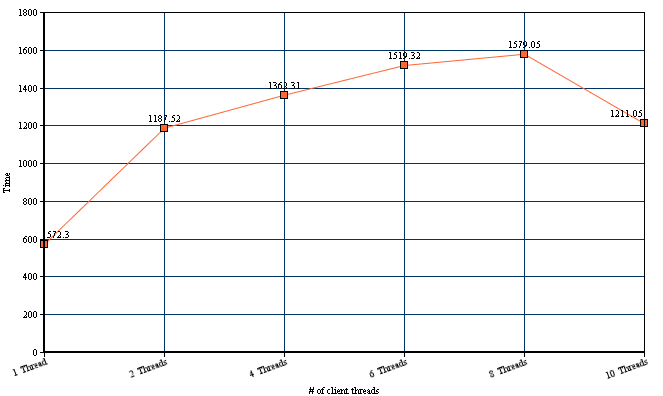
\includegraphics[scale=0.5]{images/chart1}
    \caption{Throughput(Y-axis) vs. Number of threads (X-axis)}
\end{figure}

\begin{figure}[h!]
    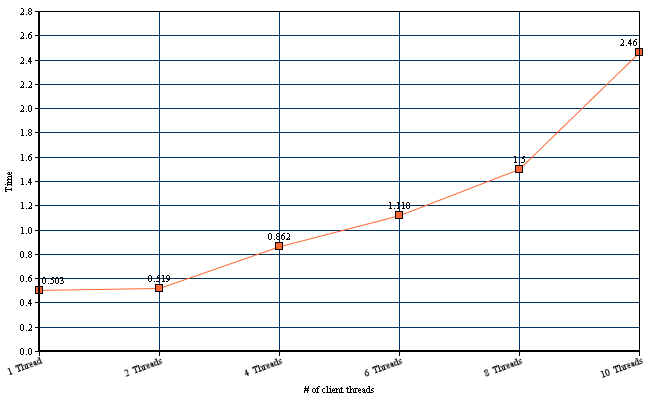
\includegraphics[scale=0.5]{images/chart2}
    \caption{Latency(Y-axis) vs. Number of threads (X-axis)}
\end{figure}

\subsection*{3}
Latency increases as expected on a local machine, linearly as the number of
workers increases. Unfortunately I was not able to get remote testing working in
time, as there were some serialization issues with XStream that I did not
resolve in time.
